% vim: tw=99

\documentclass{article}

\usepackage{fancyhdr}
\usepackage{hyperref}
\usepackage{listings}
\usepackage{minted}
\usepackage[style=nature]{biblatex}
\usepackage{booktabs}
\usepackage{tikz}
\usepackage{tkz-kiviat}
\usepackage[margin=1in]{geometry}

\usetikzlibrary{arrows}

\addbibresource{references.bib}

\providecommand*{\listingautorefname}{Listing}
\renewcommand{\sectionautorefname}{Section}

\pagestyle{fancy}
\lhead{\leftmark}
\chead{}
\rhead{}

\begin{document}

\title{ScPy: A SuperCollider Extension for Performing Numerical Computation via Embedded Python}

\author{Noah Weninger\footnote{\href{mailto:nweninge@ualberta.ca}{nweninge@ualberta.ca}}\hskip
0.75em and Abram
Hindle\footnote{\href{mailto:hindle1@ualberta.ca}{hindle1@ualberta.ca}}\\Department of Computing
Science\\University of Alberta\\Edmonton, Canada}

\maketitle

\begin{abstract}

    SuperCollider, a language for sound synthesis and algorithmic composition of audio, supports a
    wide range of synthesis, effect and analysis algorithms. However, available operations are
    limited to those implemented explicitly as Unit Generators (UGens). Since UGens are written in
    C/C++ and loaded as plugins during the SuperCollider server boot process, it is impossible to
    live code UGens, which limits the user to creating sound as a composition of existing UGens
    during a performance. Many of the vector operations required for efficiently creating complex
    audio effects are notably missing or tedious to use. To overcome this, we present ScPy, a UGen
    which embeds Python within SuperCollider to enable the use of the optimized vector operations
    provided by the NumPy library.

\end{abstract}

\section{Introduction}\label{sec:introduction}

Although a number of open-source projects which interface other languages with SuperCollider (SC)
exist~\cite{systemsinterfacingwithsc,magnusson2011ixi,orlarey2009faust}, they are mostly
SuperCollider clients, which have features to control synths and send other automation messages.
One notable exception is OctaveSC~\cite{octavesc} which embeds GNU Octave within SuperCollider.
However, it is designed for performing operations on control rate data matrices and suffers from
performance issues which prevent it from being used on audio rate data.

One of the goals of this project is to enable more flexible experimentation with FFT and phase
vocoder based operations. SuperCollider contains a total of 32 built in spectral operations
which provide the ability to produce many simple effects. There are additionally some extra
operations available as user created extensions. However, many conceivable effects are impossible,
including basic phase vocoder effects such as pitch shifting. Some examples of novel effects can
be found in~\autoref{sec:usage}.

ScPy enables users to overcome these limitations. By embedding the Python programming language
within SuperCollider, it is possible to do numerical processing operations which would be too slow
to perform in real-time with SuperCollider alone. Through access to the NumPy library, previously
difficult or impossible phase vocoder operations become trivial. Although our usage of this library
for testing purposes has mostly focused on FFT based operations, support exists for passing
arbitrary data buffers to Python, which can be used to process numerical data for many other
purposes as well.

ScPy is developed and maintained as an open-source project under the GPLv3 license. The latest
code, documentation, examples, and issues are available on
GitHub\footnote{\url{https://github.com/nwoeanhinnogaehr/ScPy}}. The code has been developed and
tested on the Linux operating system using SuperCollider version 3.6.6 and Python version 3.5.2.

\section{Literature Review}\label{sec:lit}

\subsection{NIME}

With any New Interface for Musical Expression (NIME) it is important to evaluate how it performs
and is interacted with across various dimensions. Birnbaum et al.~\cite{birnbaum2005towards}
present a new model for evaluating musical instruments by determining the position of the
instrument along 7 axes: \textit{Required Expertise}, \textit{Musical Control}, \textit{Feedback
Modalities}, \textit{Degrees of Freedom}, \textit{Inter-actors}, \textit{Distribution in Space},
and the \textit{Role of Sound}. Some of these axes represent a continuous spectrum, where as others
have discrete steps. These dimensions are arranged to form a heptagon in the 2D plane, where each
corner of the shape is placed at a distance to the center proportional to the score of the
instrument being evaluated along the corresponding axis. The specific layout of the dimensions used
in the paper additionally has properties which allow instruments of different classes to be easily
distinguished. Plots of instruments tend to occupy the right side of the graph, where as
installations tend to occupy the left. Although this model performs well on the instruments
evaluated in the paper, it is based on subjective evaluation and may accurately represent the entire
space of possible NIMEs.

ScPy is unlike many NIMEs because it is not used like any traditional musical instrument.
However, it can still be considered a NIME because it is a tool to enhance musical expression,
just with an unconventional method of interaction. A plot of ScPy in the 7-dimensional space
developed by Birnbaum et al.\ can be seen in~\autoref{fig:nime}.

\begin{figure}[ht]
    \caption{NIME dimension space analysis for ScPy.}\label{fig:nime}
    \begin{center}
        \begin{tikzpicture}[rotate=-116,xscale=-1]
            \tkzKiviatDiagram[label distance=.5cm,
                    radial=7,
                    gap=0.75,
                    lattice=4]{Required Expertise,
                    Musical Control,
                    Degrees of Freedom (Inputs),
                    Feedback Modalities (Outputs),
                    Inter-actors,
                    Distribution in Space,
                    Role of Sound}
            \tkzKiviatLine[thick,color=blue,mark=none,
                           fill=blue,opacity=.5](4,4,1.5,1.5,0.5,0.5,3)
        \end{tikzpicture}
    \end{center}
\end{figure}

Nilson~\cite{nilson2007live} presents a review of the challenges of live coding practice. Live
coding presents an interesting contrast to contemporary music with many clear differences.  While
some argue that live coding must be performed live in front of an audience, an alternate
perspective suggests that time constraints are not necessary and that the practice can refer to any
improvisational music created by programming. The practice of live coding is still quite new.
For example, Nilson writes that professional violinists will typically have practiced for 10000 hours, where
as an email survey of live coders revealed most had dedicated about 100 hours. Of course, the
prerequisite knowledge for live coding may be higher; many live coders have extensive programming
experience. Also mentioned is that the high level of abstraction offered by live coding creates a large
startup time for producing meaningful output from a blank slate. The paper presents many exercises
for improving one's live coding ability.

Nilson's work sheds light on some of the challenges faced in this project.
One such challenge is the amount of code required to produce an interesting result from a blank
slate. We intend to minimise this by providing many effect primitives and composition
mechanisms. However, it will be important to ensure the language is accessible so it can be
quickly learned to a level of expertise where lack of technical knowledge is not an impediment.

\subsection{Spectral audio processing}

The phase vocoder is an essential part of spectral audio manipulation. De G{\"o}tzen et
al.~\cite{de2000traditional} present an open source Matlab implementation along with a number of
tricks to make the implementation faster or simpler. The implementation is split into two
functions: \texttt{pv\_analyze} and \texttt{pv\_synthesize}. These functions operate as a tightly
coupled set due to the phase information maintained between frames. One of the techniques presented
is to perform a \texttt{fftshift} operation in order to simplify the phase relationship between
neighbouring bins. Another is to zero pad frames: by adding extra zeros on each side of a frame, a
larger FFT size can be used, producing better accuracy while maintaining good time resolution.

The code in this paper was used as a reference for the phase vocoder implementation in ScPy.
Additionally, some of the extra techniques mentioned could improve the quality or flexibility of
the implementation in the future.

Keiler and Sylvain~\cite{keiler2002survey} present a survey of 6 techniques for accurate analysis
of stationary sounds. The first method, plain FFT, uses a Hann window and assumes the frequencies
of the sinusoids are centered within each bin. Parabolic interpolation notices that the shape of a
magnitude peak looks like a parabola and thus attempts to fit a parabola to the magnitudes of bins
nearby each local maxima, yielding more accurate results than a plain FFT\@. The triangle algorithm
is similar to the parabolic interpolation method but fits a triangular function instead of a
parabola. Spectral reassignment uses the derivative of the analysis window to estimate the true
values of the bins as the center of gravity of the energy of each bin. The derivative algorithm
also uses the derivative of the analysis window to determine both a more accurate frequency and
amplitude. It can be further extended to use the first nth derivatives. The phase vocoder uses the
phase information of two successive FFTs to improve the frequency resolution by calculating the
phase derivative. Comparison of the techniques found that the spectral reassignment, derivative
algorithm, and phase vocoder methods had the best performance. Surprisingly, those three techniques
produced almost identical results, suggesting that they may have equivalent theoretical basis.

The two other techniques that performed similarly to the phase vocoder will be interesting to
analyze in more detail since they may present a solution to the \textit{phasiness} problem of the
phase vocoder due their lack of persistent state. However, they require extra processing so it is
not clear if the trade-off will be worthwhile.

Audio morphing is defined as a gradual change from one sound to the other. While morphing can be
achieved to some extent simply by cross fading two signals; perceptually this sounds simply like
one sound is becoming quieter as the other is becoming louder. Sethares and Bucklew
\cite{sethares2012kernel} propose density and kernel based techniques that aim to provide a more
convincing morph operation where there is no clear separation between the two sounds at any point
during the morphing process. This method allows the use of different kernel functions to provide
different kinds of morphing. These include \textit{Cross-fade}, \textit{Heat equation}, and
\textit{Harmonic integrity}. The morphing technique is implemented using a phase vocoder. These
techniques could be implemented in Python as a future extension to ScPy.

Laroche and Dolson~\cite{laroche1999improved} present an improvement to the phase vocoder which
aims to prevent the \textit{phasiness} problem where different parts of a sound lose their phase
coherence, as well as provide a significant decrease in computational cost. The paper recognizes
that there are two types of phase coherence that must be preserved in any STFT based algorithm to
ensure that the reproduced sound is without artifacts: horizontal and vertical. The basic phase
vocoder algorithm is built to preserve horizontal phase coherence but it does so at the expense
of vertical phase coherence. To remedy this, they build on prior work by presenting two new
phase-locking techniques.

Similar techniques also by Laroche and Dolson~\cite{laroche1999new} enable new phase vocoder
techniques that can be used for exotic audio effects. The core of the techniques is a peak
detection process followed by peak shifting. Since these new techniques operate on peaks the
standard phase vocoder algorithm can be simplified to not require phase unwrapping, reducing
computational complexity. Additionally, they produce better quality output than the standard phase
vocoder algorithm because of implicit phase-locking.

The phase vocoder currently implemented in ScPy uses the standard algorithm. Future experiments
could implement many of the proposed modifications to the phase vocoder to improve sound quality.

Bradford et al.\ have published a number of works detailing the sliding
DFT~\cite{bradford2005sliding} and associated sliding phase vocoder~\cite{bradford2007sliding}.
These new algorithms are efficient implementations for the STFT with a hop size of a single sample.
Although such a small hop size would be impossible to process in real-time using current hardware
and the STFT, the sliding DFT makes it possible using consumer GPU
hardware~\cite{bradford2011real}. The sliding phase vocoder additionally has a number of advantges
over traditional implementations. Quality is greatly improved but at a high computational cost. Each
analysis bin can hold any frequency, essentially making the spectrum more of a generic oscillator
bank than a traditional spectrum. This simplifies effects such as pitch shifting to a simple vector
multiplication in the frequency domain. Additionally, since the time resolution is so fine, effects
that require high resolution modulation through time such as FM or AM can now be performed in the
frequency domain.

Using Theano, the sliding DFT and sliding phase vocoder could be implemented easily in ScPy. It
remains unknown if it will be possible to run them in real-time, but even if not this future
extension could add the possibility to experiment with many novel effects.

Klingbeil~\cite{klingbeil2005software} describes the techniques used in a high quality graphical
spectral editing and resynthesis program called SPEAR\@. The FFT analysis is done taking into
account the fundamental frequency of the sound to analyze so that the transform can be optimized
to accurately capture as many partials as possible. Spectral peaks are then selected and very quiet
peaks are discarded. A linear prediction method is used to follow the peaks over time. The data
structure for storage of spectral data involves division of time into a number of frames which keep
track of which partials are active during that time so that the search for a specific partial can
be narrowed. User interface design choices are also covered in detail.

Although the interface and granularity of SPEAR differs significantly from those in ScPy, the
techniques for high quality resynthesis presented should prove useful for improving the quality of
the sound output.

While the Fourier transform is by far the most commonly used technique for spectral manipulation in
digital audio effects, there exist numerous other transformations which may be useful as well to
achieve certain audio effects. One such technique is the Mellin transform, described in a audio
effects context by De Sena and Rocchesso~\cite{de2004fast}. The Mellin transform has a scale
invariance property that is analogous to the shift invariance property of the Fourier transform. It
can be computed quickly by applying two extra steps before doing a Fourier transform: exponential
time warping and exponential multiplication. A few simple audio effects are presented using the
Mellin transform: time stretching, filtering and random phase deviation (\textit{whisperization}).

As the Mellin transform can be implemented simply as an extension to the Fourier transform, it
should be fairly easy to add support for it in ScPy and it will hopefully enable the use of
some different audio effects than can be achieved easily with the Fourier transform. However, the
paper mentions that a short-time Mellin transform has not been attempted, so some further work may
need to be done in that area first.

\subsection{Lanugages}

Collins et al.~\cite{collins2003live} present an introduction to the field of live coding where
code to generate sound is written live during a performance, often on a laptop computer. Although
the use graphical programming environments such as Reaktor, Pure Data, or MAX/MSP in live
performances is in some sense live coding, the paper focuses on the use of text based programming
environments. Many of the pros and cons of live coding are presented. Although live coding adds
some very interesting new possibilities to live music performance, it is not without its
challenges. Case studies of two live coding environments are included: Slub and SuperCollider with
the \textit{just in time} library.

ScPy can be used for live coding of audio effects similarly to how the environments studied in
this paper can be used to live code synths and pattens. More details about how ScPy was designed to
facilitate this can be found in \autoref{sec:methodology}.

Domain-Specific Languages (DSLs) are small programming languages designed for use in a specific
problem domain. They often lack general purpose programming constructs and have a syntax which is
very concise for describing programs in their domain. Van Deursen et al.~\cite{van2000domain}
present a survey of available DSL literature, along with the pros and cons of using a DSL, example
DSLs, design methodology and implementation approaches. The biggest advantage of DSLs is that they
enable expression of solutions in a way that is common for the problem domain. However, they can be
costly to develop and difficult to design. Implementation techniques include the classical approach
of interpretation or compilation, embedded languages / domain-specific libraries, preprocessing, or
compiler extension. The paper also includes an annotated bibliography.

This review presents many useful ideas for language design within ScPy. Although we decided not to
design a DSL for our project, analyzing the design and implementation techniques presented here
will be helpful for future work in this area.

As Python is an easily extendible general purpose language, it has applications in many scientific
fields. Glover et al.~\cite{glover2011python} present a discussion of the use of Python for audio
signal processing. They note that while audio processing libraries exist for many languages,
scripting languages such as Python or MATLAB see widespread adoption because of the speed at which
prototypes can be built. General purpose Python libraries such as NumPy, SciPy and Matplotlib
include many essential functions for audio processing, such as file IO, Fourier transforms, signal
processing and interpolation. There are additionally more specific libraries such as Simpl, a
sinusoidal modelling library, and Modal, an onset detection library. Any of these libraries can
easily be used within ScPy simply by installing and importing them.

Another audio related open-source Python library is librosa~\cite{mcfee2015librosa} by McFee et
al.\ librosa is a music signal analysis library designed to help transition music information
retrieval (MIR) researchers into using Python, as well as make MIR techniques readily available to
all Python programmers.\ librosa's core design choices and conventions are documented in detail to
inspire future library authors to follow similarly good coding practice. As well as standard audio
analysis functions, librosa also includes support for effects and audio IO.\@

librosa has quite an extensive list of features and would likely cover all of the audio related
functionality which is missing from NumPy. It can be used with ScPy simply by installing and importing
it.

The ixi lang~\cite{magnusson2011ixi} by Magnusson is a live coding language. It is implemented as an interpreter
built in SuperCollider, a choice which allows for SuperCollider and ixi lang code to be mixed
together in a similar manner to ScPy. The ixi lang is built to reduce the startup time in a live
coding performance and enable faster musical experimentation through syntax more concise than
SuperCollider. This paper also contains user feedback on the usability of the ixi lang.

Since the ixi lang is similar to ScPy in many ways, many of the design choices made in ixi lang are
also appropriate in ScPy. Lessons learned from the user feedback for ixi lang could
potentially be used to improve the usability of ScPy.

\section{Methodology}\label{sec:methodology}

During the initial planning stage of the project, we wanted to provide a set of fundamental
operations on spectral data which could be composed together to perform any conceivable effect. It
was also a requirement that these operations would be syntactically concise to enable easy and fast
experimentation. Ideally, the system would be able to handle complex effects in real-time.

The choice of SuperCollider was largely because it is one of the most widely used audio programming
environments. Using SuperCollider also enabled the reuse of many parts of its code base. Since it
already has STFT based operations, it was a good target for extension purposes in that area.

Although designing a domain-specific language for this task was briefly considered, we eventually
decided to use Python for a number of reasons. First, Python includes an excellent C API which
makes embedding it within other languages trivial in comparison to many other options. Second,
Python's syntax is easily readable and concise and therefore it adheres to our goals.  Finally,
Python has a massive number of community built libraries for performant scientific and numerical
computing. With a few small exceptions, which are clearly specific to spectral data (such as the
phase vocoder), these libraries contained every one of the fundamental operations we could think
of.

It may seem as though embedding an interpreted language within an interpreted language could offer
no performance advantage. There is certainly some loss of performance when switching languages and
transferring data. However, the biggest advantage comes not strictly from performance but from the
diversity of operations which become available with highly optimized implementations. NumPy is used
internally by ScPy for handling data arrays so the entire NumPy library of mathematical functions
comes at no cost. Any other Python library can easily be imported as well. Limited experiments
have been done with the SciPy library. It would also be possible to use Theano to do processing on
the GPU for extra performance. Implementing an equivalent to these popular Python libraries in pure
SuperCollider is certainly possible, but it would require a very large amount of work and would see
no adoption outside of the audio computing community.

In order to facilitate the use of ScPy in live coding performances, many errors are ignored or
handled in a way that can be easily recovered from. In particular, floating point errors such as
division by zero or other invalid operations are ignored. Special values such as infinity or NaN
are replaced with zeros. This is done because SuperCollider has poor handling of these special
values and in some cases will crash if they are found. Python exceptions are printed to the
SuperCollider post window, where they can easily be examined and corrected by the user.

\section{Usage}\label{sec:usage}

Use of ScPy is through the classes \texttt{Py}, \texttt{PyOnce}, \texttt{PyFile}, and
\texttt{PyOnceFile}. \texttt{Py} is used for processing real-time data and \texttt{PyOnce} is used
for doing initialization or other one time processing. Both have one required argument: a block of
Python code. The \texttt{PyFile} and \texttt{PyOnceFile} variants take a filename instead of inline
code. For all classes, a map of variable names may optionally be provided to bind SuperCollider
variables to Python variables. Additionally, there is an optional \texttt{DoneAction} argument
which specifies an action to occur in SuperCollider after the Python code has finished executing.

\begin{listing}[ht]
    \begin{minted}[linenos=true]{SuperCollider}
PyOnce("print('Hello from Python!')");
    \end{minted}
    \caption{Hello world with ScPy.}
    \label{lst:helloworld}
\end{listing}

\begin{listing}[ht]
    \inputminted[linenos=true]{SuperCollider}{../examples/template.sc}
    \caption{SuperCollider boilerplate for no-op FFT effect with ScPy.}
    \label{lst:boilerplate}
\end{listing}

When \autoref{lst:boilerplate} is run, an anonymous synth is created which will take in audio
from an external source, perform an STFT, process the spectral data with ScPy, perform an inverse
STFT, then finally output the resulting audio. Lines 8--9 contain Python code defining the
processing function where operations are to be inserted. Further examples will replace only those
lines. Line 16 contains the Python code to convert the spectrum into a NumPy array, process it,
then write back the processed version.

A special function, \texttt{out}, is provided to mutate data in SuperCollider buffers. It takes a
variable which is bound to a \texttt{Buffer} or \texttt{FFT} object and a new value. The buffer is
modified in place to hold the new data.

Complex numbers are used extensively, even to represent non-Cartesian data such as polar
coordinates or phase vocoder bins in ScPy. In polar form, the real and imaginary parts represent
magnitude and phase, respectively. Similarly for the phase vocoder, real and imaginary parts
represent magnitude and frequency. This is done to take advantage of the limited data types
available in NumPy and relative convenience of working with complex numbers as opposed to tuples or
classes. Future work could extend NumPy to give more descriptive names to these data fields.

\begin{listing}[ht]
    \begin{minted}[linenos=true]{python}
pv = PhaseVocoder(hop)

def fn(x):
    x = pv.forward(x)
    idx = indices(x.shape)[1]
    x = pv.shift(x, lambda freq:
        freq * (0.8 + mod(-time + 0.1*idx, 10)*0.045))
    x = pv.backward(x)
    return x
    \end{minted}
    \caption{A novel effect to transform any sound into a falling Shepard tone. This example makes
    use of the phase vocoder \texttt{shift} operation, which applies a function to frequency, then
    reorganizes the spectrum to move the new frequencies into the appropriate bins.}
    \label{lst:shepard}
\end{listing}

\begin{listing}[ht]
    \begin{minted}[linenos=true]{python}
pv = PhaseVocoder(hop)

def fn(x):
    x = pv.forward(x)
    x = pv.to_bin_offset(x)
    x.imag *= -1 # imaginary part holds frequency
    x = pv.from_bin_offset(x)
    x = pv.backward(x)
    return x
    \end{minted}
    \caption{An effect which inverts the frequency of each analysis bin across the center of
    the bin, creating an unusual detuning effect.}
    \label{lst:binflipper}
\end{listing}

\section{Implementation}\label{sec:implementation}

\begin{figure}[ht]
    \caption{A high level overview of data flow and processing.}
    \begin{center}
        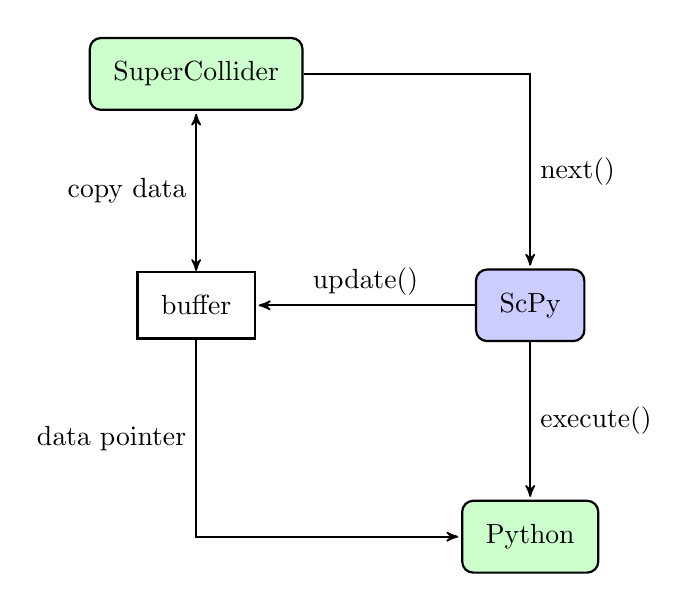
\begin{tikzpicture}[
            every matrix/.style={ampersand replacement=\&,column sep=2cm,row sep=2cm},
            sink/.style={draw,thick,rounded corners,fill=green!20,inner sep=.3cm},
            process/.style={draw,thick,rounded corners,fill=blue!20,inner sep=.3cm},
            datastore/.style={draw,thick,inner sep=.3cm},
            to/.style={->,>=stealth',shorten >=1pt,semithick},
            both/.style={<->,>=stealth',shorten >=1pt,semithick},
            every node/.style={align=center}]

            \matrix{\node[sink] (sc) {SuperCollider}; \\
                    \node[datastore] (objects) {buffer}; \& \node[process] (scpy) {ScPy}; \\
                    \& \node[sink] (py) {Python}; \\
            };

            \draw[to] (sc) -| node[near end,right] {next()} (scpy);
            \draw[to] (objects) |- node[near start,left] {data pointer} (py);
            \draw[both] (objects) -- node[midway,left] {copy data} (sc);
            \draw[to] (scpy) -- node[midway,right] {execute()} (py);
            \draw[to] (scpy) -- node[midway,above] {update()} (objects);
        \end{tikzpicture}
    \end{center}
\end{figure}

ScPy is written mostly in C++, but with a small SuperCollider class library to connect the C++
back-end and a small Python library that provides some useful operations. Due to differences
between these languages, connecting them was somewhat awkward in some cases.

Since UGens may only be used as part of a synth, \texttt{PyOnce} is provided as a wrapper which
hides this detail from the user and allows the execution of Python code outside of a synth. It
internally just starts a synth with the \texttt{doneAction} argument set such that the synth
terminates after running once.

One issue involves the process of passing data between SuperCollider and C++. Since UGens are
designed to work primarily with data streams, adding support for passing in many types of data came
with a number of challenges. Essentially, all data must be serialized into an array of floats.
Strings must be converted to an array of ASCII character codes and prepended with their length.
Arguments passed through to the Python code can have one of many types and therefore type
information must be encoded as well. However, just passing the type of a variable is not enough to
know what we can do with it, since we also want to know if it inherits from a class we can use. The
encoding and decoding implementation is unfortunately fairly complex, but creating a UGen with
inputs this complicated was likely not considered during the design of SuperCollider, so some
friction was expected in this area.

Since \texttt{FFT} objects in SuperCollider operate on a single channel only they must be placed
in \texttt{Array} objects to support multichannel audio. \texttt{Array}s can hold objects of any
type, so it is natural to convert them to Python \texttt{list} objects, which have similar
properties. However, this presents an interesting problem: multichannel \texttt{FFT} objects are
then converted to \texttt{list}s of \texttt{ndarray} objects in Python. These are a bit more
awkward to work with than basic \texttt{ndarray} objects, but can easily be converted using a call
to the \texttt{array} function in Python. This can be seen in practice on line 16 of
\autoref{lst:boilerplate}. Although it would be possible to do this conversion
automatically it is left out for the purpose of not introducing a feature simply to work around an
incomplete implementation of \texttt{FFT} objects in SuperCollider. The current conversions will
continue to function as intended if \texttt{FFT} objects are given multichannel support in the
future.

Control UGens only provide a single floating point value per cycle so it would seem natural to
convert them to a Python \texttt{float}, but in ScPy they are instead transferred to Python in a
one element \texttt{ndarray}. This is because Python provides no numerical types with interior
mutability. In practice, NumPy accepts a one element \texttt{ndarray} almost anywhere a
\texttt{float} is accepted, so this detail is usually not an annoyance.

\begin{table}[ht]
    \caption{Type correspondence between SuperCollider and Python}
    \begin{center}
        \begin{tabular}{ll}
            \toprule
            SuperCollider type & Python type \\
            \midrule
            \texttt{Float} & \texttt{float} \\
            (subclass of) \texttt{UGen} & \texttt{ndarray} of \texttt{float} \\
            \texttt{Buffer} & \texttt{ndarray} of \texttt{float} \\
            \texttt{FFT} & \texttt{ndarray} of \texttt{complex} \\
            \texttt{Array} & \texttt{list} \\
            \bottomrule
        \end{tabular}
    \end{center}
\end{table}

As shown in \autoref{lst:shepard} and \autoref{lst:binflipper}, ScPy includes a phase vocoder
implemented in Python for performing frequency transformations. Interestingly, although all of
SuperCollider's FFT operations are referred to as phase vocoder operations in the code and
documentation, there is actually no implementation of a phase vocoder to be found in the
SuperCollider code base at the time of writing. It is likely that a phase vocoder was once intended
to be implemented, but the 32 so-called phase vocoder effects are simply transformations to the
Cartesian or polar representations of the spectrum.

\section{Future Work}

At the time of writing, ScPy only supports handling audio rate data via SuperCollider's
\texttt{Buffer} objects. In order to make some use cases more ergonomic ScPy could certainly be
extended to support raw audio rate input. This would make time domain audio data even
simpler to work with than frequency domain data is currently. It would also enable SuperCollider's
FFT UGen to be easily re-implemented in Python for greater flexibility.

Support for more SuperCollider types, such as events or strings, could be added to open up ScPy to
more use cases. Adding support for more types should be trivial in the existing code base.

Multi-core processing support would allow for many more sounds to be processed in real-time.
Currently, all processing is done on a single thread even with many UGens running at once. Using
the supernova server~\cite{blechmann2005supernova} may be helpful however it has not yet been
tested and ScPy may require some modifications to be usable with supernova.

Creating a more generic extension which supports many languages would have a number of advantages.
Although extending SuperCollider was the focus of this project, similar improvements could be made
to the CSound~\cite{boulanger2000csound,lazzarini2005extensions}, Chuck~\cite{wang2008chuck} or
Faust~\cite{orlarey2009faust} environments as well. It may be desirable to completely separate the
embedded language from the host in order to allow easier interoperation and a cleaner
implementation.

Throughout~\autoref{sec:lit}, articles are discussed which contain processing techniques that could
be used in ScPy. Although implementations of many of these techniques may to become a part of ScPy
in the future, there is no obstacle to the reader implementing them as external Python libraries
usable by ScPy.

\section{Conclusion}

While the number of possible future extensions to ScPy is numerous, the basic implementation that
currently exists is more than enough to yield countless exotic and novel audio effects. In the
limited experiments that we did using the software, it was found to be very easy to produce many
advanced sounds, thanks to the excellent documentation and implementation of the Python language
and NumPy library. Although it was possible to make these effects without our technology, ScPy
makes it possible to experiment with them at an unprecedented rate and listen to their output in
real-time.

Initial tests have been promising but they have so far have been focused on spectral processing,
leaving time domain audio and control rate data processing largely untested. Further experiments in
these areas could reveal previously unknown new use cases.

Those that wish to experiment with ScPy should note that the code may contain bugs due to the
infancy of the project and the nonstandard ways we are interfacing with SuperCollider. It is our
intention to maintain and improve this project in the future. Users are encouraged to submit bug
reports on the project's GitHub page\footnote{\url{https://github.com/nwoeanhinnogaehr/ScPy}}.

\printbibliography{}

\end{document}
